\section{RF Design Practices}
{\color{sub}\footnotesize 10 hrs \gap$\cdot$\gap asked in \mk{all 24 papers}
\gap$\cdot$\gap 3 syllabus sub-topics \gap$\cdot$\gap \mk{426 marks, 22.4\% of the archive,
the heaviest chapter}
$\rightarrow$ one filter question and one amplifier numerical in almost every paper.}

\vspace{3pt}\noindent
\colorbox{gdL}{\makebox[\dimexpr\textwidth-2\fboxsep][l]{%
  \textcolor{gd}{\bfseries\footnotesize READ THIS FIRST}}}
\par\nobreak\vspace{3pt}

Chapter 6 is worth about 18 marks a paper and it is \mk{two fixed questions}:
\begin{enumerate}[label=\arabic*., leftmargin=1.4em, itemsep=1pt]
  \item \textbf{A filter question} (20 of 24 papers): ``why the insertion loss method'',
    ``how is a Butterworth / Chebyshev LPF prototyped'', ``design steps'', then ``sketch
    it in microstrip''. $\rightarrow$ $\S$6.1 to $\S$6.3. The theory is one page; the
    marks are in the \textbf{procedure} and the \textbf{layout sketch}.
  \item \textbf{An amplifier numerical} (22 papers, 10 to 18 marks): a transistor's four
    S-parameters, ``check stability and compare maximum gain for bilateral and unilateral
    modes''. $\rightarrow$ theory $\S$6.4, every PYQ set solved in the companion. The papers
    \textbf{attach the formula sheet}; what they mark is the order of the steps and the
    arithmetic.
\end{enumerate}
Two things worth knowing before the paper starts:
\begin{itemize}
  \item Of the 13 distinct S-parameter sets in the archive, \mk{three are not
    unconditionally stable} (the $0.894\angle{-60.6^\circ}$ set in 4 papers, 76 Bh, 73 Ma).
    For those a ``bilateral maximum gain'' does not exist and the answer must say so. The
    companion shows what to write instead.
  \item Oscillator and mixer theory are asked in only 2 papers each, as short notes
    ($\S$6.5, $\S$6.6).
\end{itemize}

\hr

%=======================================================================
\T{6.1 Microwave Filters and the Insertion Loss Method}

\Q{Why are microwave filters designed using the insertion loss method? How is a Butterworth / Chebyshev LPF prototyped?}{\m{4}\m{5}\m{2+6}\m{3+5}\m{6+2}\m{8}\m{10}}
{\color{sub}\footnotesize \tS{20} \yr{\textbf{70 Bh}, 70 Ma, 71 Bh, \textbf{72 Ash}, 72 Ma, \textbf{73 Bh}, 73 Ma, \textbf{74 Bh}, 74 Ma, \textbf{75 Bh}, \textbf{76 Bh}, \textbf{77 Ch}, \textbf{78 Ch}, \textbf{\texttt{79 Bh}}, \texttt{80 Ba}, \textbf{\texttt{80 Bh}}, \texttt{81 Ba}, \textbf{\texttt{81 Bh}}, \texttt{82 Ba}, \textbf{\texttt{82 Bh}}} \gap$\cdot$\gap \mk{the most repeated ask in the chapter}}

\sbs{%
\lead{Filters, and the two design methods}
\begin{itemize}
  \item \textbf{Filter}: two-port that passes a frequency band and attenuates the rest:
    LPF, HPF, BPF, BSF.
  \item \textbf{Image parameter method} (1930s): cascade simple sections with the right
    cut-off and attenuation.
  \begin{itemize}
    \item Cannot specify the \textbf{whole} response; needs repeated iteration.
  \end{itemize}
  \item \textbf{Insertion loss method (ILM)}: network synthesis from a specified
    \textbf{power loss ratio} over all frequencies.
\end{itemize}}{%
\lead{Power loss ratio}
\[ P_{LR} = \frac{P_{\text{available}}}{P_{\text{load}}} = \frac{1}{1 - |\Gamma(\omega)|^2}
   = 1 + \frac{M(\omega^2)}{N(\omega^2)} \]
\begin{itemize}
  \item $|\Gamma|^2$ is even in $\omega$, so $M$, $N$ are polynomials in $\omega^2$.
  \item Insertion loss $IL = 10\log P_{LR}$ dB; matched both ends:
    $P_{LR} = 1/|S_{21}|^2$.
\end{itemize}}

\sbs{%
\lead{Why the insertion loss method (the 2 to 3 mark answer)}
\begin{itemize}
  \item Response is \textbf{completely specified} and met exactly, no trial and error.
  \item Explicit trade-offs: \textbf{binomial} for minimum passband loss,
    \textbf{Chebyshev} for sharpest cut-off, \textbf{linear phase} for low distortion.
  \item Order $N$ follows from the stopband requirement.
  \item Starts from \textbf{normalised low-pass prototypes} ($R_0 = 1\,\Omega$,
    $\omega_c = 1$ rad/s), so one table serves every filter after scaling.
  \item Designs improve systematically with $N$; CAD tools implement it directly.
\end{itemize}
\figT{c6_responses.png}
{\color{sub}\scriptsize $N = 3$: equal-ripple is sharper, maximally flat is smoother.
Gangaju Ch-6 deck, slide 11.}}{%
\lead{The three standard responses}
\begin{itemize}
  \item \textbf{Maximally flat (Butterworth, binomial)}:
    $P_{LR} = 1 + k^2(\omega/\omega_c)^{2N}$.
  \begin{itemize}
    \item Band-edge loss $1 + k^2$; $k = 1$ gives $-3$ dB.
    \item Beyond cut-off rises $20N$ dB/decade; flattest possible passband.
  \end{itemize}
  \item \textbf{Equal ripple (Chebyshev)}: $P_{LR} = 1 + k^2T_N^2(\omega/\omega_c)$.
  \begin{itemize}
    \item Ripple of amplitude $1 + k^2$ in the passband.
    \item Also $20N$ dB/decade, but $\dfrac{2^{2N}}{4}$ times more attenuation than
      Butterworth well beyond cut-off.
  \end{itemize}
  \item \textbf{Linear phase}: $\phi = A\omega[1 + p(\omega/\omega_c)^{2N}]$, maximally
    flat group delay; poorer selectivity.
\end{itemize}}

\par\penalty0\Needspace{18\baselineskip}
\sbsr{0.52}{%
\lead{Low-pass prototype and element values}
\figT{c6_ladder.png}
{\color{sub}\scriptsize The two dual ladder forms, $g_0 = 1$ source, $g_{N+1}$ load. Deck
slide 7 (Pozar p.403).}
\begin{itemize}
  \item \textbf{Butterworth} ($k = 1$): $g_k = 2\sin\dfrac{(2k-1)\pi}{2N}$, $g_{N+1} = 1$.
  \item \textbf{Chebyshev}, ripple $L_r$ dB: $\beta = \ln\coth\frac{L_r}{17.37}$,
    $\gamma = \sinh\frac{\beta}{2N}$, $a_k = \sin\frac{(2k-1)\pi}{2N}$,
    $b_k = \gamma^2 + \sin^2\frac{k\pi}{N}$;
    $g_1 = \dfrac{2a_1}{\gamma}$, $g_k = \dfrac{4a_{k-1}a_k}{b_{k-1}g_{k-1}}$;
    $g_{N+1} = 1$ for odd $N$, $\coth^2\frac{\beta}{4}$ for even $N$.
  \item \textbf{Order} (Butterworth): smallest $N$ with
    $10\log\left[1 + (\omega/\omega_c)^{2N}\right] \ge$ required stopband loss.
\end{itemize}}{%
\lead{Tables (computed in \code{filt.py}, equal to Pozar's)}
{\footnotesize
\begin{tabularx}{\linewidth}{@{}L{0.5cm}XXXXXX@{}}
\toprule
\hrow \thead{$N$} & \thead{$g_1$} & \thead{$g_2$} & \thead{$g_3$} & \thead{$g_4$} & \thead{$g_5$} & \thead{$g_6$} \\
\midrule
\multicolumn{7}{@{}l}{\textbf{Maximally flat}} \\
1 & 2.0000 & 1.0000 & & & & \\
2 & 1.4142 & 1.4142 & 1.0000 & & & \\
3 & 1.0000 & 2.0000 & 1.0000 & 1.0000 & & \\
4 & 0.7654 & 1.8478 & 1.8478 & 0.7654 & 1.0000 & \\
5 & 0.6180 & 1.6180 & 2.0000 & 1.6180 & 0.6180 & 1.0000 \\
\midrule
\multicolumn{7}{@{}l}{\textbf{Equal ripple, 0.5 dB}} \\
1 & 0.6987 & 1.0000 & & & & \\
2 & 1.4029 & 0.7071 & 1.9841 & & & \\
3 & 1.5963 & 1.0967 & 1.5963 & 1.0000 & & \\
4 & 1.6704 & 1.1925 & 2.3662 & 0.8419 & 1.9841 & \\
5 & 1.7058 & 1.2296 & 2.5409 & 1.2296 & 1.7058 & 1.0000 \\
\midrule
\multicolumn{7}{@{}l}{\textbf{Equal ripple, 3.0 dB}} \\
1 & 1.9954 & 1.0000 & & & & \\
2 & 3.1014 & 0.5339 & 5.8095 & & & \\
3 & 3.3489 & 0.7117 & 3.3489 & 1.0000 & & \\
4 & 3.4391 & 0.7483 & 4.3473 & 0.5920 & 5.8095 & \\
5 & 3.4815 & 0.7619 & 4.5378 & 0.7619 & 3.4815 & 1.0000 \\
\bottomrule
\end{tabularx}}
\begin{itemize}
  \item Deck example: 20 dB at 4 GHz for $f_c = 2.5$ GHz. The deck (via Pozar's chart)
    takes $N = 6$ (24.5 dB); the formula shows $N = 5$ already gives 20.4 dB. $N = 6$ is
    safe, just not minimal. \added{}
\end{itemize}}

\par\penalty0\Needspace{10\baselineskip}
\creamq{Why are Butterworth and Chebyshev common to prototype two-port filters?}{\m{4}}
{\color{sub}\footnotesize \yr{\textbf{70 Bh}, 70 Ma}}
\begin{itemize}
  \item Both power loss ratios are \textbf{polynomials} in $\omega^2$ that give a
    \textbf{realisable lossless LC ladder} with closed-form element values.
  \item They sit at the two ends of the useful trade-off: \textbf{flattest passband}
    (Butterworth) vs \textbf{sharpest cut-off} for a given $N$ (Chebyshev).
  \item Tabulated, normalised values mean a designer only \textbf{scales}; the same table
    gives LPF, HPF, BPF and BSF by transformation ($\S$6.2).
  \item Ladders map directly onto transmission-line sections, so both are practical in
    microstrip ($\S$6.3).
\end{itemize}

\penalty0\vspace{2pt}

%=======================================================================
\T{6.2 Filter Design Steps: Scaling and Conversion}

\Q{Explain the steps of microwave filter design; how is a LPF prototype converted to other filters?}{\m{5}\m{6+4}\m{7+3}\m{3+8+3}\m{10}}
{\color{sub}\footnotesize same papers as $\S$6.1 \gap$\cdot$\gap 71 Bh, 72 Ma, 74 Bh, \texttt{80 Bh}, \texttt{81 Ba}, \texttt{82 Ba}, \texttt{82 Bh} ask the steps outright}

\sbs{%
\lead{The procedure (write it as four boxes)}
\begin{enumerate}[label=\arabic*., leftmargin=1.4em, itemsep=1pt]
  \item \textbf{Specifications}: type, cut-off $f_c$ (or band $f_1$ to $f_2$), passband
    loss or ripple, stopband attenuation at a stated frequency, $R_0$.
  \item \textbf{Low-pass prototype}: choose response, find $N$, read $g_1$ to $g_{N+1}$
    ($R_0 = 1$, $\omega_c = 1$).
  \item \textbf{Scaling and conversion}: impedance-scale by $R_0$, frequency-scale to
    $\omega_c$, and transform LP $\rightarrow$ HP / BP / BS.
  \item \textbf{Implementation}: lumped (below about 5 GHz) or distributed microstrip:
    stepped impedance, Richards' stubs, Kuroda identities ($\S$6.3).
\end{enumerate}
\lead{Impedance and frequency scaling (LPF)}
\[ L'_k = \frac{R_0L_k}{\omega_c}, \qquad C'_k = \frac{C_k}{R_0\omega_c},
   \qquad R'_s = R'_L = R_0 \]}{%
\figT{c6_transform.png}
{\color{sub}\scriptsize Element transformations, $\Delta = (\omega_2 - \omega_1)/\omega_0$,
$\omega_0 = \sqrt{\omega_1\omega_2}$. Deck slide 19 (Pozar p.414).}
\lead{Conversion rules}
\begin{itemize}
  \item \textbf{LPF $\rightarrow$ HPF}, $\omega \rightarrow -\omega_c/\omega$: series L
    becomes series C $= \dfrac{1}{R_0\omega_cL_k}$; shunt C becomes shunt L
    $= \dfrac{R_0}{\omega_cC_k}$.
  \item \textbf{LPF $\rightarrow$ BPF}: series L $\rightarrow$ series LC
    ($L_k R_0/\omega_0\Delta$, $\Delta/\omega_0L_kR_0$); shunt C $\rightarrow$ shunt LC
    ($\Delta R_0/\omega_0C_k$, $C_k/\omega_0\Delta R_0$).
  \item \textbf{LPF $\rightarrow$ BSF}: the reverse pairing (series arms become parallel
    LC, shunt arms series LC).
\end{itemize}}

\par\penalty0\Needspace{11\baselineskip}
\creamq{Worked scaling check: Butterworth $N = 3$, $f_c = 2.5$ GHz, $R_0 = 50\,\Omega$}{}
\begin{tabularx}{\linewidth}{@{}L{2.2cm}L{3.7cm}L{3.7cm}X@{}}
\toprule
\hrow \thead{Prototype} & \thead{LPF element} & \thead{HPF element} & \thead{Check (ABCD in \code{filt.py})} \\
\midrule
$g_1 = 1$ (shunt) & $C_1 = \frac{1}{50\times2\pi\times2.5\text{e}9} = 1.27$ pF & shunt $L = \frac{50}{\omega_c} = 3.18$ nH & \\
$g_2 = 2$ (series) & $L_2 = \frac{50\times2}{\omega_c} = 6.37$ nH & series $C = \frac{1}{50\omega_c\times2} = 0.637$ pF & $|S_{21}| = -3.01$ dB at 2.5 GHz, both \\
$g_3 = 1$ (shunt) & $C_3 = 1.27$ pF & shunt $L = 3.18$ nH & \\
\bottomrule
\end{tabularx}

\penalty0\vspace{2pt}

%=======================================================================
\T{6.3 Microstrip Implementation}

\Q{Implement the filter using microstrip: LPF $\pi$ / double $\pi$, double-pad T-type, double-section shunt-arm or series-arm, HPF, single-section series-arm BPF}{\m{2}\m{3}\m{3+5}\m{5+3}\m{7+3}\m{8+2}\m{10}}
{\color{sub}\footnotesize \tS{13} \yr{\textbf{72 Ash}, 73 Ma, \textbf{74 Bh}, 74 Ma, \textbf{76 Bh}, \textbf{78 Ch}, \textbf{\texttt{79 Bh}}, \texttt{80 Ba}, \textbf{\texttt{80 Bh}}, \texttt{81 Ba}, \textbf{\texttt{81 Bh}}, \texttt{82 Ba}, \textbf{\texttt{82 Bh}}} \gap$\cdot$\gap the sketch carries the marks; label every section}

\sbsr{0.50}{%
\lead{Why microstrip, and the two methods}
\begin{itemize}
  \item Lumped L, C work to about 5 GHz; above that their size and spacing are no
    longer small in wavelengths.
  \item Microstrip: planar, cheap, light, easy to mount active devices; but lossier,
    lower power, radiates and couples.
  \item \textbf{Stepped impedance} (Hi-Z / Low-Z): alternate very high and very low
    impedance short lines.
  \item \textbf{Stubs} (Richards' transformation): inductor $\rightarrow$ short-circuited
    stub, capacitor $\rightarrow$ open-circuited stub, each $\lambda/8$ long at $f_c$;
    Kuroda identities separate series stubs.
\end{itemize}
\lead{Why a short line is an L or a C}
\begin{itemize}
  \item T-model of a line length $l$: series $X/2 = Z_0\tan(\beta l/2)$, shunt
    $B = \sin(\beta l)/Z_0$.
  \item \textbf{High} $Z_0$, short: $X \approx Z_h\beta l$, $B \approx 0$
    $\rightarrow$ a \textbf{series inductor}.
  \item \textbf{Low} $Z_0$, short: $B \approx \beta l/Z_l$, $X \approx 0$
    $\rightarrow$ a \textbf{shunt capacitor}.
  \item Design lengths:
    \[ \beta l = \frac{g_kR_0}{Z_h}\ \text{(inductor)}, \qquad
       \beta l = \frac{g_kZ_l}{R_0}\ \text{(capacitor)} \]
    Keep $\beta l < 45^\circ$; typically $Z_h \approx 100$ to $120\,\Omega$,
    $Z_l \approx 20\,\Omega$.
\end{itemize}}{%
\figT{c6_stepped_deck.png}
{\color{sub}\scriptsize Stepped-impedance LPF and its layout. Deck slide 26.}
\vspace{2pt}

\figT{c6_elliptic.png}
{\color{sub}\scriptsize Elliptic LPF with capacitive stubs alternating sides to cut
cross-talk. Deck slide 27.}
\begin{itemize}
  \item \textbf{Checked}: \code{filt.py} reproduces the deck's example table
    ($N = 6$, $Z_h = 120$, $Z_l = 20\,\Omega$, $\epsilon_r = 4.2$, $h = 1.58$ mm):
    $\beta l = 11.8, 33.8, 44.3, 46.1, 32.4, 12.3^\circ$, $W = 11.3$ and
    $0.43$ mm.
\end{itemize}}

\par\penalty0\Needspace{12\baselineskip}
\lead{Vocabulary the papers use}
\begin{itemize}
  \item \textbf{Pad}: a wide, low-$Z$ section = a \textbf{shunt capacitor}.
  \item \textbf{Series arm}: an element in the signal path (series L in an LPF, series C in
    an HPF). \textbf{Shunt arm}: an element to ground (shunt C as a pad or open stub; shunt
    L as a shorted stub).
  \item \textbf{$\pi$-section}: shunt, series, shunt (C-L-C for a LPF).
    \textbf{T-section}: series, shunt, series (L-C-L).
  \item \textbf{Double / triple}: two or three such sections cascaded.
\end{itemize}
{\color{sub}\footnotesize The layouts below are drawn \textbf{to scale} by \code{filt.py} from
computed dimensions for one assumed specification, which is what a paper that says
``illustrate an example'' expects: Butterworth, $f_c = 2.5$ GHz, $R_0 = 50\,\Omega$,
$Z_h = 120\,\Omega$, $Z_l = 20\,\Omega$, $\epsilon_r = 4.2$, $h = 1.58$ mm ($W_{50} = 3.13$ mm).}

\par\penalty0\Needspace{14\baselineskip}
\sbs{%
\lead{LPF $\pi$-section, $N = 3$ (79 Bh, 73 Ma, 74 Ma, 72 Ash)}
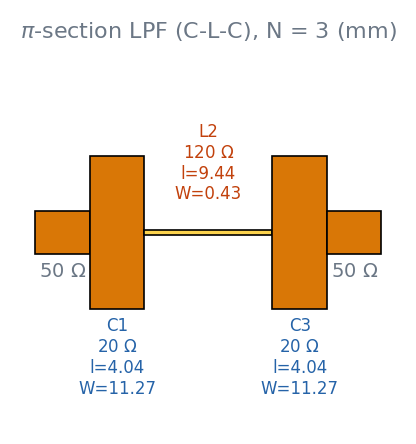
\includegraphics[width=\linewidth,height=3.3cm,keepaspectratio]{figs/c6_lay_pi3.png}
\begin{itemize}
  \item $g = 1, 2, 1$: pads $\beta l = 22.9^\circ$ (4.04 mm), line $47.7^\circ$ (9.44 mm).
\end{itemize}}{%
\lead{Double $\pi$-section, $N = 5$ (76 Bh)}
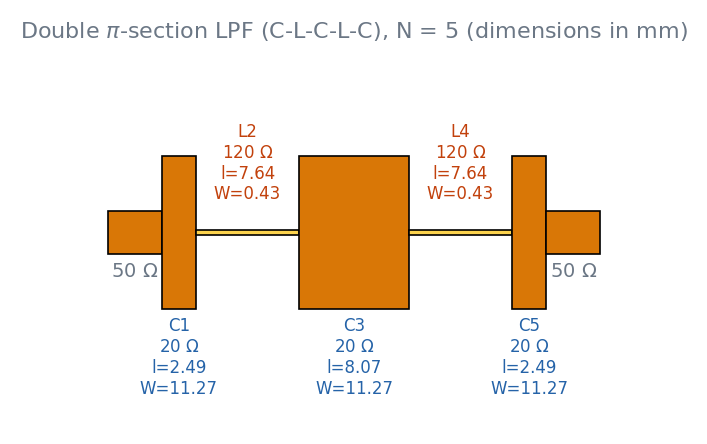
\includegraphics[width=\linewidth,height=3.3cm,keepaspectratio]{figs/c6_lay_pi5.png}
\begin{itemize}
  \item $g = 0.618, 1.618, 2, 1.618, 0.618$: three pads, two high-$Z$ lines.
\end{itemize}}

\par\penalty0\Needspace{14\baselineskip}
\sbs{%
\lead{Double-pad T-type, $N = 5$ (\texttt{81 Ba}; series-arm, 78 Ch)}
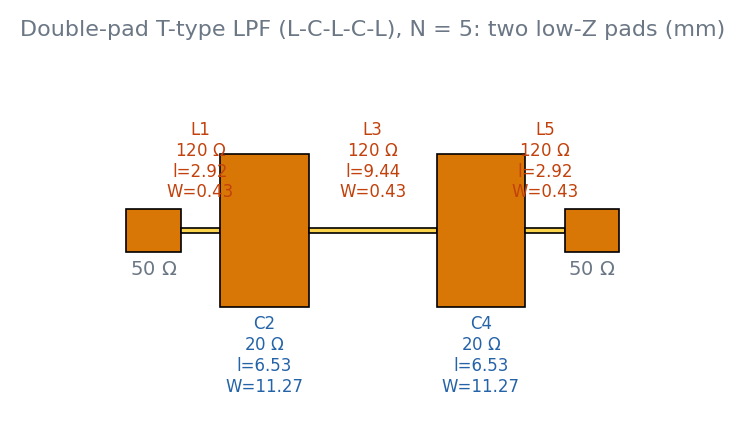
\includegraphics[width=\linewidth,height=3.3cm,keepaspectratio]{figs/c6_lay_t5.png}
\begin{itemize}
  \item L-C-L-C-L: the \textbf{series arms} are the three high-$Z$ lines, the two
    \textbf{pads} the shunt capacitors. A ``double-section series-arm'' filter is this
    layout.
\end{itemize}}{%
\lead{Double-section shunt-arm LPF, $N = 4$ (\texttt{80 Ba})}
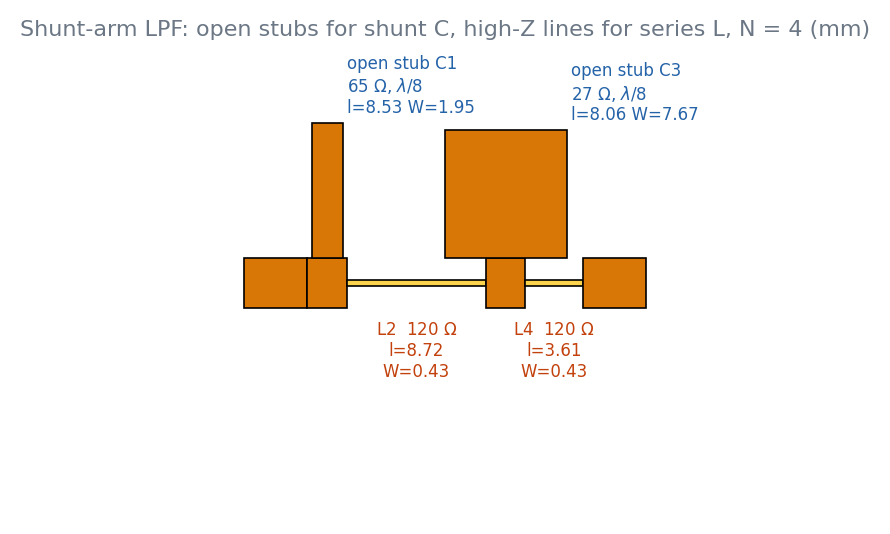
\includegraphics[width=\linewidth,height=3.3cm,keepaspectratio]{figs/c6_lay_stub.png}
\begin{itemize}
  \item Shunt capacitors as \textbf{open stubs}, $\lambda/8$ at $f_c$ with
    $Z = R_0/g_k$ (Richards): 65 and 27 $\Omega$; series inductors as high-$Z$ lines.
\end{itemize}}

\par\penalty0\Needspace{14\baselineskip}
\sbs{%
\lead{HPF $\pi$-section (74 Bh, \texttt{80 Bh}, \texttt{82 Ba})}
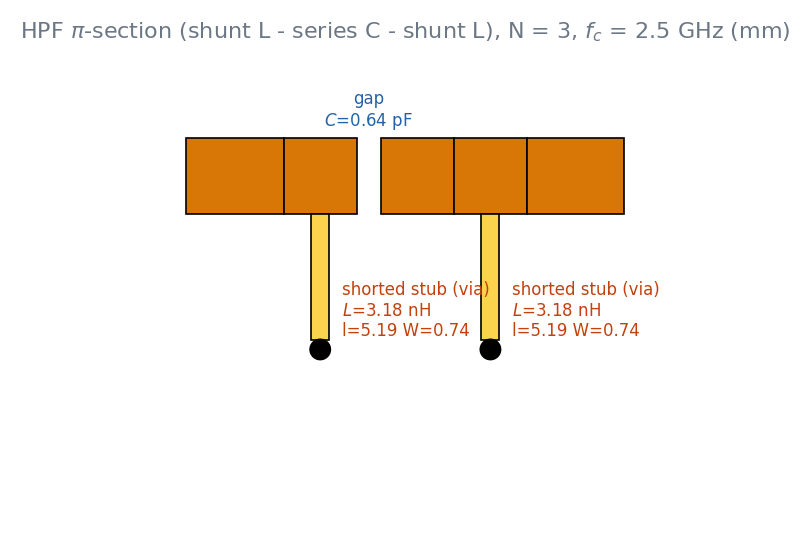
\includegraphics[width=\linewidth,height=3.3cm,keepaspectratio]{figs/c6_lay_hpf.png}
\begin{itemize}
  \item From the C-L-C prototype: shunt $L = 3.18$ nH, series $C = 0.637$ pF.
  \item Series capacitor = a \textbf{gap} (or interdigital) in the strip; shunt inductor =
    a \textbf{short-circuited stub} through a via: $Z_s\tan\beta l = \omega_cL$ gives
    5.19 mm of $100\,\Omega$ line.
  \item \textbf{Triple-pad series-arm HPF} (\texttt{82 Ba}): three pads separated by two
    gaps (the series capacitors) with shorted stubs from the pads.
  \item \texttt{80 Bh}'s ``second-order $\pi$'': one series gap between two stubbed pads.
\end{itemize}}{%
\lead{Single-section series-arm BPF (\texttt{81 Bh})}
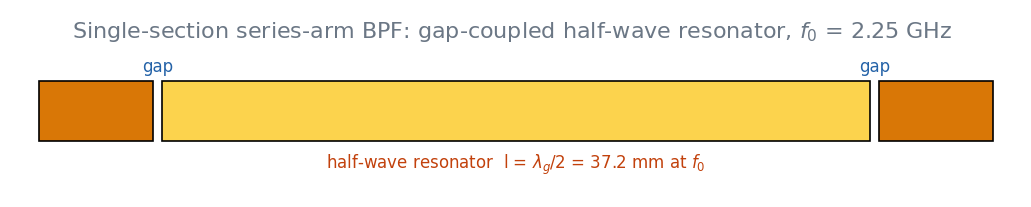
\includegraphics[width=\linewidth,height=3.3cm,keepaspectratio]{figs/c6_lay_bpf.png}
\begin{itemize}
  \item The series LC arm of a BPF is a \textbf{half-wave resonator} coupled by a gap at
    each end: resonant at $f_0$ (series-resonant, passes), capacitively coupled (blocks
    DC and low frequencies).
  \item $l = \lambda_g/2$ at $f_0$: 37.2 mm on 50 $\Omega$ at 2.25 GHz.
  \item More sections (more resonators) sharpen the skirts.
\end{itemize}}

\penalty0\vspace{2pt}

%=======================================================================
\T{6.4 RF Amplifier Theory: Gain, Stability and Design Flow}

\Q{Draw the design flowchart of a microwave amplifier; stability analysis; stability synthesis on the Smith chart; amplifier vs oscillator}{\m{4}\m{5}\m{3+8}\m{5+5}\m{6+4}\m{8}\m{10}}
{\color{sub}\footnotesize \tS{10} \yr{71 Bh, 71 Ma, \textbf{73 Bh}, \textbf{74 Bh}, \textbf{75 Bh}, \textbf{76 Bh}, \textbf{78 Ch}, \texttt{81 Ba}, \textbf{\texttt{81 Bh}}, \texttt{82 Ba}} \gap$\cdot$\gap the theory half of the amplifier questions}

\sbs{%
\lead{Reflection coefficients seen by the device}
\[ \Gamma_{in} = S_{11} + \frac{S_{12}S_{21}\Gamma_L}{1 - S_{22}\Gamma_L}
   = \frac{S_{11} - \Delta\Gamma_L}{1 - S_{22}\Gamma_L} \]
\[ \Gamma_{out} = S_{22} + \frac{S_{12}S_{21}\Gamma_S}{1 - S_{11}\Gamma_S}
   = \frac{S_{22} - \Delta\Gamma_S}{1 - S_{11}\Gamma_S} \]
{\color{sub}\footnotesize $\Delta = S_{11}S_{22} - S_{12}S_{21}$. From $b_2 = S_{21}a_1 + S_{22}\Gamma_Lb_2$ (deck slides 33 to 34).}
\lead{Three power gains}
\begin{itemize}
  \item \textbf{Transducer} $G_T = P_L/P_{avs}$ (the one the papers use).
  \item \textbf{Available} $G_A = P_{avn}/P_{avs}$; \textbf{operating}
    $G_P = P_L/P_{in}$.
\end{itemize}
\[ G_T = \frac{1 - |\Gamma_S|^2}{|1 - \Gamma_{in}\Gamma_S|^2}\,|S_{21}|^2\,
         \frac{1 - |\Gamma_L|^2}{|1 - S_{22}\Gamma_L|^2} \]
\begin{itemize}
  \item \textbf{Unilateral} ($S_{12} \approx 0$): $G_{TU} = G_S\,G_0\,G_L$ with
    $G_0 = |S_{21}|^2$; maximum at $\Gamma_S = S_{11}^*$, $\Gamma_L = S_{22}^*$:
    \[ G_{TU,max} = \frac{1}{1 - |S_{11}|^2}\,|S_{21}|^2\,\frac{1}{1 - |S_{22}|^2} \]
  \item \textbf{Unilateral figure of merit}
    $M = \dfrac{|S_{11}||S_{12}||S_{21}||S_{22}|}{(1 - |S_{11}|^2)(1 - |S_{22}|^2)}$;
    error bound $\dfrac{1}{(1 + M)^2} < \dfrac{G_T}{G_{TU}} < \dfrac{1}{(1 - M)^2}$.
    Unilateral is acceptable if the bound is a few tenths of a dB.
  \item \textbf{Bilateral maximum} (simultaneous conjugate match,
    $\Gamma_S = \Gamma_{in}^*$, $\Gamma_L = \Gamma_{out}^*$), only if unconditionally stable:
    \[ \Gamma_S = \frac{B_1 - \sqrt{B_1^2 - 4|C_1|^2}}{2C_1}, \quad
       \Gamma_L = \frac{B_2 - \sqrt{B_2^2 - 4|C_2|^2}}{2C_2} \]
    $B_1 = 1 + |S_{11}|^2 - |S_{22}|^2 - |\Delta|^2$, $C_1 = S_{11} - \Delta S_{22}^*$ (and
    $1 \leftrightarrow 2$). Then
    $G_{T,max} = \dfrac{|S_{21}|}{|S_{12}|}\left(K - \sqrt{K^2 - 1}\right)$.
\end{itemize}}{%
\lead{Stability}
\begin{itemize}
  \item \textbf{Oscillation} is possible if $|\Gamma_{in}| > 1$ or $|\Gamma_{out}| > 1$
    (negative resistance at a port).
  \item \textbf{Unconditionally stable}: $|\Gamma_{in}|, |\Gamma_{out}| < 1$ for
    \textbf{every} passive source and load. Test (Rollett):
    \[ K = \frac{1 - |S_{11}|^2 - |S_{22}|^2 + |\Delta|^2}{2|S_{12}S_{21}|} > 1
       \ \text{and}\ |\Delta| < 1 \]
    or the single test $\mu = \dfrac{1 - |S_{11}|^2}{|S_{22} - \Delta S_{11}^*| + |S_{12}S_{21}|} > 1$.
  \item \textbf{Conditionally (potentially) stable}: some $\Gamma_S$ or $\Gamma_L$ cause
    oscillation. Find them with \textbf{stability circles}:
    \[ C_L = \frac{(S_{22} - \Delta S_{11}^*)^*}{|S_{22}|^2 - |\Delta|^2}, \quad
       R_L = \left|\frac{S_{12}S_{21}}{|S_{22}|^2 - |\Delta|^2}\right| \]
    \[ C_S = \frac{(S_{11} - \Delta S_{22}^*)^*}{|S_{11}|^2 - |\Delta|^2}, \quad
       R_S = \left|\frac{S_{12}S_{21}}{|S_{11}|^2 - |\Delta|^2}\right| \]
  \item On the \textbf{output circle} $|\Gamma_{in}| = 1$; on the \textbf{input circle}
    $|\Gamma_{out}| = 1$. Each is a boundary, not a region.
\end{itemize}
\figT{c6_stab_circles.png}
{\color{sub}\scriptsize Deck slides 45 to 46: $S_{11} = 0.65\angle{-95^\circ}$ etc. at 800 MHz,
$K = 0.547$: $C_S = 1.79\angle122^\circ$, $R_S = 1.04$; $C_L = 1.30\angle48^\circ$,
$R_L = 0.45$. Hatched overlaps are the unstable $\Gamma$. Reproduced exactly in
\code{amp.py}.}}

\par\penalty0\Needspace{16\baselineskip}
\sbs{%
\lead{Which side of the circle is stable (synthesis on the Smith chart)}
\begin{enumerate}[label=\arabic*., leftmargin=1.4em, itemsep=1pt]
  \item Plot $C_L$, $R_L$ (and $C_S$, $R_S$) on the chart.
  \item Test the \textbf{centre} $\Gamma_L = 0$: there $|\Gamma_{in}| = |S_{11}|$.
  \item If $|S_{11}| < 1$ the centre is stable, so the stable region is the side of the
    circle that contains the centre:
  \begin{itemize}
    \item $|C_L| > R_L$ (centre outside) $\Rightarrow$ stable \textbf{outside} the circle.
    \item $|C_L| < R_L$ (centre inside) $\Rightarrow$ stable \textbf{inside}.
  \end{itemize}
  \item Same for the source circle with $|S_{22}|$.
  \item Circle entirely outside the unit chart (or enclosing it on the stable side)
    $\Rightarrow$ unconditionally stable. Circle cutting the chart $\Rightarrow$
    conditionally stable; choose $\Gamma_S$, $\Gamma_L$ well inside the stable part.
\end{enumerate}
{\color{sub}\footnotesize 73 Bh, 74 Bh, 75 Bh give a sketched chart; 71 Bh gives the circles
directly. Worked: companion Problem 7.}}{%
\lead{Amplifier design flowchart (write as boxes joined by arrows)}
\begin{enumerate}[label=\arabic*., leftmargin=1.4em, itemsep=1pt]
  \item \textbf{Specify} $f$, gain, noise figure, $Z_0$; \textbf{choose a transistor}
    (GaAs FET / HEMT / BJT) and bias; read its S-parameters.
  \item \textbf{Stability}: compute $\Delta$, $K$ (or $\mu$).
  \item $K > 1$, $|\Delta| < 1$? \textbf{Yes} $\rightarrow$ step 4. \textbf{No}
    $\rightarrow$ draw stability circles, restrict $\Gamma_S$, $\Gamma_L$ to the stable
    region (or add resistive loading / feedback), then step 4.
  \item \textbf{Unilateral check}: compute $M$ and the error bound.
  \begin{itemize}
    \item Small $\rightarrow$ $\Gamma_S = S_{11}^*$, $\Gamma_L = S_{22}^*$ (or gain
      circles for a specified gain).
    \item Large $\rightarrow$ bilateral: $\Gamma_S$, $\Gamma_L$ from $B$, $C$.
  \end{itemize}
  \item \textbf{Gain}: $G_{TU,max}$ or $G_{T,max}$; compare with the specification.
  \item \textbf{Matching networks}: realise $\Gamma_S$ and $\Gamma_L$ from $50\,\Omega$
    with a line plus a stub (Smith chart, Ch 2).
  \item \textbf{Bias network}, DC blocks, RF chokes; \textbf{layout} in microstrip;
    simulate, build, measure, tune.
\end{enumerate}
\figT{c6_amp_final.png}
{\color{sub}\scriptsize Final amplifier: input network, transistor, output network. Deck
slide 58.}}

\par\penalty0\Needspace{11\baselineskip}
\creamq{Amplifier circuit vs oscillator circuit in terms of stability factor}{\m{5}}
{\color{sub}\footnotesize \yr{71 Ma}}
\begin{tabularx}{\linewidth}{@{}L{2.6cm}XX@{}}
\toprule
\hrow & \thead{Amplifier} & \thead{Oscillator} \\
\midrule
Wanted & stable: no self-oscillation & unstable: oscillation on purpose \\
Stability factor & $K > 1$ and $|\Delta| < 1$ (or $\mu > 1$), or $\Gamma_S$, $\Gamma_L$ kept in the stable region & $K < 1$: device potentially unstable \\
Port reflection & $|\Gamma_{in}|, |\Gamma_{out}| < 1$ & $|\Gamma_{in}| > 1$ (negative resistance) \\
Terminations & conjugate match for gain & $\Gamma_S$ chosen \textbf{inside} the unstable region; $\Gamma_{in}\Gamma_S = 1$, $\Gamma_{out}\Gamma_L = 1$ \\
Input signal & required & none; starts from noise \\
Feedback & avoided, or negative & positive, loop gain $A\beta \ge 1$ \\
\bottomrule
\end{tabularx}

\par\penalty0\Needspace{8\baselineskip}
\Q{Stability and maximum gain numericals (bilateral and unilateral)}{\m{5+5}\m{10}\m{12}\m{15}\m{18}}
{\color{sub}\footnotesize \tS{22} \yr{69 Bh, \textbf{70 Bh}, 70 Ma, 71 Bh, 71 Ma, \textbf{72 Ash}, 72 Ma, 73 Ma, \textbf{74 Bh}, 74 Ma, \textbf{76 Bh}, \textbf{77 Ch}, \textbf{78 Ch}, \textbf{\texttt{79 Bh}}, \textbf{79 Ch}, \texttt{80 Ba}, \textbf{\texttt{80 Bh}}, \textbf{80 Ch}, \texttt{81 Ba}, \textbf{\texttt{81 Bh}}, \texttt{82 Ba}, \textbf{\texttt{82 Bh}}} \gap$\cdot$\gap \mk{every set is solved in the companion}}
\begin{itemize}
  \item 13 distinct S-parameter sets across 22 papers; the companion works one in full,
    tabulates the rest with every intermediate, and splits out the cases that need a
    different answer (conditionally stable, given terminations, full matching design,
    circles given directly).
\end{itemize}

\penalty0\vspace{2pt}

%=======================================================================
\T{6.5 Microwave Oscillator Theory}

\Q{Microwave oscillator theory}{\m{8}}
{\color{sub}\footnotesize \tP{2} \yr{70 Ma, 71 Ma} \gap$\cdot$\gap 71 Ma as the amplifier-vs-oscillator contrast of $\S$6.4}

\sbsr{0.56}{%
\lead{Feedback view}
\begin{itemize}
  \item Gain $A$ with positive feedback $\beta$: $\dfrac{e_o}{e_i} = \dfrac{A}{1 - A\beta}$.
  \item $A\beta = 1$ $\rightarrow$ finite output with no input: \textbf{Barkhausen
    condition}. To start, $A\beta \approx 1.1$ to $1.2$; oscillation grows from noise until
    gain compression brings $A\beta$ back to 1.
\end{itemize}
\lead{Negative-resistance view (the microwave one)}
\begin{itemize}
  \item A device port with $|\Gamma_{out}| > 1$ has \textbf{negative resistance}.
  \item \textbf{One-port oscillator}: device $Z_{out} = R_{out} + jX_{out}$ with
    $R_{out} < 0$, load $Z_L$. Loop condition $\Gamma_{out}\Gamma_L = 1$ gives
    \[ R_L + R_{out} = 0, \qquad X_L + X_{out} = 0 \]
  \item To start oscillation the circuit must have net negative resistance:
    $R_L < |R_{out}|$. The deck's rule $|R_{out}| \ge 1.2R_L$ (Pozar uses
    $R_L = |R_{out}|/3$).
  \item \textbf{Two-port oscillator}: transistor with a \textbf{generator tuning network}
    ($\Gamma_S$) and a \textbf{load network} ($\Gamma_L$). Conditions:
    \begin{enumerate}[label=\arabic*., leftmargin=1.4em, itemsep=0pt]
      \item $K < 1$: device potentially unstable.
      \item $\Gamma_{in}\Gamma_S = 1$.
      \item $\Gamma_{out}\Gamma_L = 1$ (equivalent to 2, shown by substituting
        $\Gamma_{in}$).
    \end{enumerate}
\end{itemize}}{%
\figT{c6_feedback.png}
{\color{sub}\scriptsize Positive feedback. Deck slide 60.}
\vspace{2pt}

\figT{c6_twoport_osc.png}
{\color{sub}\scriptsize Two-port oscillator. Deck slide 62.}
\vspace{2pt}

\figT{c6_oneport.png}
{\color{sub}\scriptsize One-port: negative-resistance device and load. Deck slide 65.}}

\par\penalty0\Needspace{14\baselineskip}
\sbsr{0.62}{%
\lead{Two-port design steps}
\begin{enumerate}[label=\arabic*., leftmargin=1.4em, itemsep=1pt]
  \item From the S-parameters find $K$; need $K < 1$ (use a common-gate / common-base
    configuration or series feedback to make it so).
  \item Draw the \textbf{input stability circle}.
  \item Choose $\Gamma_S$ \textbf{inside the unstable region}, usually on the rim for the
    largest $|\Gamma_{out}|$; realise it with an inductor or shorted stub.
  \item $\Gamma_{out} = S_{22} + \dfrac{S_{12}S_{21}\Gamma_S}{1 - S_{11}\Gamma_S}$,
    $|\Gamma_{out}| > 1$ $\rightarrow$ $Z_{out} = R_{out} + jX_{out}$ with $R_{out} < 0$.
  \item Choose $R_L = |R_{out}|/3$ (start-up margin), $X_L = -X_{out}$; design the load
    matching network.
\end{enumerate}
\lead{Worked: Gunn diode one-port (deck slide 66, checked in \code{amp.py})}
\begin{itemize}
  \item $\Gamma_{out} = 1.24\angle30^\circ$ at 10 GHz. Plot $1/\Gamma_{out}^* = 0.806\angle30^\circ$,
    read $z$ and negate the real part: $Z_{out} = -68.9 + j159.0\,\Omega$ (deck reads
    $-70 + j160$).
  \item Resonance: $X_L = -159\,\Omega$, a capacitor $C = 1/(2\pi f\cdot159) = 0.100$ pF.
  \item Start-up: \textbf{the deck picks $R_L = 60\,\Omega$, which breaks its own rule}:
    $|R_{out}| \ge 1.2R_L$ needs $R_L \le 57.5\,\Omega$. Use $R_L = 23\,\Omega$ (Pozar's
    $|R_{out}|/3$) or at most $57\,\Omega$. \added{}
\end{itemize}}{%
\figT{c6_osc_steps.png}
{\color{sub}\scriptsize $\Gamma_S$ chosen inside the input stability circle. Deck slide 67.}
\lead{Oscillator types and stabilisation}
\begin{itemize}
  \item Transistor (FET, BJT), Gunn, IMPATT (one-port); YIG-tuned (wide tuning), DRO
    (dielectric resonator, low phase noise).
  \item Frequency stability: high-Q resonator in the tuning network; isolator at the
    output (Ch 4).
\end{itemize}}

\penalty0\vspace{2pt}

%=======================================================================
\T{6.6 Microwave Mixer}

\Q{Mixer theory / microwave mixer}{\m{5}}
{\color{sub}\footnotesize \tP{2} \yr{\textbf{70 Bh}, 72 Ma} \gap$\cdot$\gap \added{} the deck has no mixer slides; written from Pozar Ch 13}

\begin{itemize}
  \item \textbf{Mixer}: a \textbf{nonlinear} three-port (diode or FET) that multiplies an
    RF signal $f_{RF}$ with a local oscillator $f_{LO}$ to translate it in frequency.
  \item Square-law principle: $i = a v^2$ with $v = V_{RF}\cos\omega_{RF}t + V_{LO}\cos\omega_{LO}t$
    contains $aV_{RF}V_{LO}\cos(\omega_{RF} \pm \omega_{LO})t$: \textbf{sum and difference}
    (checked by FFT in \code{amp.py}).
  \item \textbf{Down-conversion}: keep $f_{IF} = |f_{RF} - f_{LO}|$ with a filter; the
    \textbf{superheterodyne} receiver then amplifies at a fixed IF.
  \item \textbf{Up-conversion} (transmitters): keep $f_{RF} = f_{LO} + f_{IF}$.
  \item \textbf{Image frequency}: $f_{IM} = f_{LO} \pm f_{IF}$ on the other side of the LO
    also lands on $f_{IF}$ $\rightarrow$ reject it with an RF pre-filter or an
    image-reject mixer.
  \item \textbf{Figures of merit}: conversion loss $L_c = 10\log(P_{RF}/P_{IF})$
    (typically 4 to 7 dB for diode mixers), noise figure, LO-RF and LO-IF isolation,
    1 dB compression, intermodulation.
  \item \textbf{Types}:
  \begin{itemize}
    \item \textbf{Single-ended diode}: one Schottky diode; simple, poor isolation.
    \item \textbf{Balanced}: two diodes fed through a 90$^\circ$ or 180$^\circ$ hybrid
      (magic tee, rat race, Ch 4): cancels LO AM noise, better isolation, better input
      match.
    \item \textbf{Double-balanced}: diode ring with two baluns: suppresses even
      harmonics and both RF and LO at the IF port.
    \item \textbf{FET mixers}: conversion \textbf{gain} instead of loss.
  \end{itemize}
\end{itemize}

\penalty0\vspace{2pt}

%=======================================================================
\T{6.7 PYQ Mapping}

\lead{Theory questions, covered in this document}
\begin{itemize}
  \item \textbf{Insertion loss method; why it is used} $\rightarrow$ $\S$6.1.
    \yr{\textbf{72 Ash} \m{5}, \textbf{73 Bh} \m{2+6}, 73 Ma \m{8}, \textbf{75 Bh} \m{5},
    \texttt{80 Ba} \m{3}, \textbf{\texttt{81 Bh}} \m{8}, \textbf{\texttt{82 Bh}} \m{3}}
  \item \textbf{Butterworth and Chebyshev common to prototype filters} $\rightarrow$ $\S$6.1.
    \yr{\textbf{70 Bh} \m{4}, 70 Ma \m{4}}
  \item \textbf{LPF prototyping (Butterworth, Chebyshev); filter parameters}
    $\rightarrow$ $\S$6.1. \yr{\textbf{72 Ash} \m{5}, 72 Ma \m{5}, 74 Ma \m{3}, \textbf{76 Bh} \m{8},
    \textbf{77 Ch} \m{8}, \textbf{\texttt{79 Bh}} \m{6}, \textbf{\texttt{80 Bh}} \m{10}}
  \item \textbf{Filter design steps; conversion to other filter types} $\rightarrow$ $\S$6.2.
    \yr{71 Bh \m{5}, \textbf{74 Bh} \m{6}, \textbf{\texttt{80 Bh}} \m{10}, \texttt{81 Ba} \m{7},
    \texttt{82 Ba} \m{7}, \textbf{\texttt{82 Bh}} \m{8}}
  \item \textbf{Microstrip implementation} (LPF $\pi$, double $\pi$, double-pad T, shunt-arm,
    series-arm, HPF, BPF) $\rightarrow$ $\S$6.3. \yr{\textbf{72 Ash} \m{3}, 73 Ma \m{2},
    \textbf{74 Bh} \m{4}, 74 Ma \m{5}, \textbf{76 Bh} \m{2}, \textbf{78 Ch} \m{10},
    \textbf{\texttt{79 Bh}} \m{2}, \texttt{80 Ba} \m{5}, \textbf{\texttt{80 Bh}} \m{10},
    \texttt{81 Ba} \m{3}, \textbf{\texttt{81 Bh}} \m{2}, \texttt{82 Ba} \m{3}, \textbf{\texttt{82 Bh}} \m{3}}
  \item \textbf{Design steps of a given 5th-order ladder (figure)} $\rightarrow$ companion
    Problem 10. \yr{\textbf{\texttt{82 Bh}} \m{3+8+3}}
  \item \textbf{Amplifier design flowchart} $\rightarrow$ $\S$6.4. \yr{71 Bh \m{5},
    \textbf{73 Bh} \m{10}, \textbf{74 Bh} \m{4}, \textbf{76 Bh} \m{4}, \textbf{78 Ch} \m{10},
    \texttt{81 Ba} \m{3}, \textbf{\texttt{81 Bh}} \m{3}, \texttt{82 Ba} \m{4}}
  \item \textbf{Stability analysis; synthesis from a sketched Smith chart} $\rightarrow$
    $\S$6.4 and companion Problem 7. \yr{\textbf{73 Bh} \m{10}, \textbf{74 Bh} \m{8},
    \textbf{75 Bh} \m{5}, \texttt{81 Ba} \m{4}, \texttt{82 Ba} \m{4}}
  \item \textbf{Stability of given circles $C_S, R_S, C_L, R_L$} $\rightarrow$ companion
    Problem 7. \yr{71 Bh \m{5}}
  \item \textbf{Amplifier vs oscillator in terms of stability factor} $\rightarrow$ $\S$6.4.
    \yr{71 Ma \m{5}}
  \item \textbf{Microwave oscillator theory} $\rightarrow$ $\S$6.5. \yr{70 Ma \m{8}}
  \item \textbf{Mixer theory} $\rightarrow$ $\S$6.6. \yr{\textbf{70 Bh} \m{5}, 72 Ma \m{5}}
\end{itemize}

\lead{Numerical content}
\begin{itemize}
  \item \textbf{This chapter has a numerical companion}, \textit{Ch6 - RF Design Practices -
    Numerical Problems and Solutions}: every amplifier S-parameter set in the archive
    (22 papers) and the 82 Bh filter design. All values from \code{src/amp.py} and
    \code{src/filt.py}.
\end{itemize}

\lead{Errors found and corrected}
\begin{itemize}
  \item Deck slide 51 (8 GHz example): $|\Delta| = 0.168$, $K = 3.53$; exactly
    $0.173$ and $3.445$ (verdict unchanged).
  \item Deck slide 52: $M = 0.04$ and bounds $-0.36$ to $+0.37$ dB; exactly $M = 0.034$,
    $-0.29$ to $+0.30$ dB.
  \item Deck slide 66: $R_L = 60\,\Omega$ violates the deck's own start-up rule.
  \item Deck example 8.6: $N = 5$ already meets 20 dB; $N = 6$ is conservative.
  \item Sorted PYQ documents: 71 Ma's set and marks, 70 Ma and 80 Ba asks, the missing
    75 Bh Smith-chart question and 72 Ma mixer note (fixed before this chapter).
\end{itemize}
